%- block legend
Dado dois números inteiros $A$ e $B$, determine o valor de $A + B$.

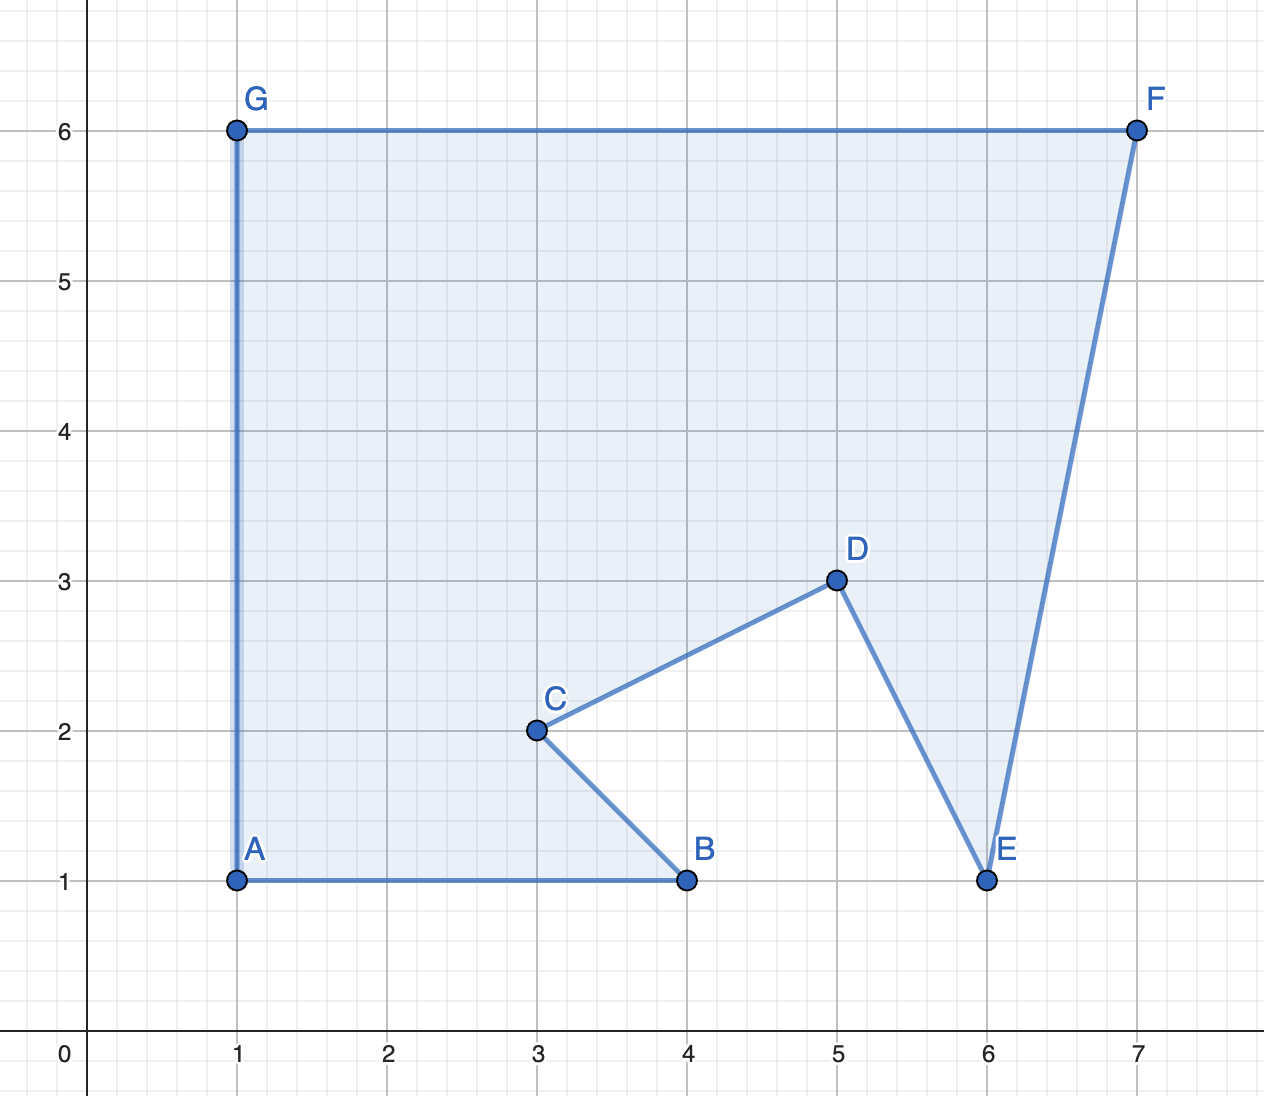
\includegraphics[width=6cm]{projecao.png}
%- endblock

%- block input
A entrada é composta por uma única linha contendo dois números
inteiros $A$ e $B$ ($1 \leq A, B \leq \VAR{vars.MAX_N | sci}$).
%- endblock

%- block output
A saída deve conter somente um único inteiro, a soma de $A$ e $B$.
%- endblock

%- block notes
Adicione aqui explicações pros exemplos, ou remova este bloco caso não seja necessário.
%- endblock
